\problemname{Släktträffen}
\begin{figure}[h!]
  \centering
  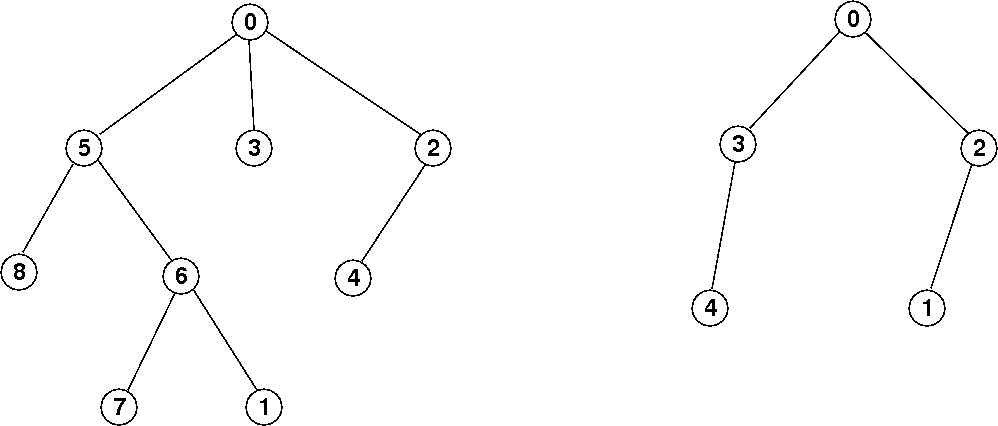
\includegraphics[width=16cm]{slakttraffen.png}
  \caption{Släktträden för de två körningsexemplen.}
\end{figure}

Det är släktträff för ättlingar till Ida-Ottilia Isaksson.
För enkelhets skull har man upprättat ett släktträd och numrerat alla ättlingarna från $1$ till $N$, samt givit Ida-Ottilia själv numret $0$.
Bland de M personerna vid ditt bord uppkommer en diskussion om vem som är er närmaste gemensamma släkting (uppåt i trädet).
Skriv ett program som räknar ut detta.

Programmet ska fråga efter antalet ättlingar, $N$, och därefter fråga efter numret på varje persons förälder, vilket naturligtvis alltid är mellan $0$ och $N$.
Därefter ska programmet fråga efter antalet personer vid bordet, M ($2 \le M \le N$), och läsa in numret på var och en av dem.
Programmet ska skriva ut numret på den person som är närmast gemensam släkting (uppåt i trädet) till alla vid bordet.
Observera att detta ibland kan vara någon vid bordet.

\section*{Indata}
På första raden i indata står talen $N$ och $M$ ($2 \le M \le N \le 20$).
På andra raden står $N$ tal, föräldrarna för varje ättling (alla mellan $0$ och $N$).
På tredje raden står $M$ tal, personerna runt bordet (alla mellan $1$ och $N$, utan dubbletter).

\section*{Utdata}
Programmet ska skriva ut ett enda tal: numret på personernas närmaste gemensamma släkting.
